% +------------------------------------------------------------------------+
% | CGAL Reference Manual:  qt_widget.tex
% +------------------------------------------------------------------------+
% | Using Qt_widget to visualize CGAL Objects
% | 
% |
% |
% | 12.12.2001  Radu Ursu
% | 
\RCSdef{\qtwidgetRev}{$Revision$}
\RCSdefDate{\qtwidgetDate}{$Date$}
% +------------------------------------------------------------------------+

\newcommand{\qt}{{\em Qt}}      %QT abbreviation

\gdef\lciIfHtmlClassLinks{\lcFalse}
\gdef\lciIfHtmlRefLinks{\lcFalse}
\gdef\lciIfHtmlLinks{\lcFalse}

\chapter{Qt\_widget}
\label{chapterQtwidget}

\ccChapterRelease{\qtwidgetRev. \ \qtwidgetDate}\\
\ccChapterAuthor{Radu Ursu}


\begin{figure}[h]
\begin{ccTexOnly}
\begin{center}
\includegraphics{../doc_tex/support/Qt_widget/triangulation.eps} 
\end{center}
\end{ccTexOnly}
\begin{ccHtmlOnly}
<CENTER>
<IMG BORDER=0 SRC="../doc_tex/support/Qt_widget/triangulation.gif"  ALIGN=center  ALT="A Nice Screen Shoot">
</CENTER>
\end{ccHtmlOnly}
\end{figure}
\begin{table}[h]
\end{table}

\qt\ is a {\sc Gui} toolkit\footnote{http://www.trolltech.com} for
cross-platform application development. 

% +-----------------------------------------------------+
\section{Introduction}

In this chapter we describe a widget and some helper classes that
allow to interact with two dimensional \cgal\ objects in \qt\/ based applications.

The most important class is the class \ccStyle{Qt_widget}. It provides
a drawing area and output stream operators for \cgal\ objects, as well
as zooming and panning functionality.

The \ccStyle{Qt_widget} allows to attach {\em layers}. Layers usually
draw on the drawing area of the widget. Layers can be activated and
deactivated, and what you see in the drawing area is the overlay of
all attached activated layers. Layers can be used also for entering
input, and \cgal\ provides input \ccc{layers} for the two-dimensional
\cgal\ objects.

Finally, we provide a {\em toolbar} for controlling the basic functionality
of the \ccStyle{Qt_widget}.

The following sections describe the main class as well as the helper classes
in more detail and give examples that can be taken as starting points for
new applications.


\section{Qt\_widget}
\label{Qt_widget}

The class \ccStyle{Qt_widget} is derived from the \qt\ class \ccStyle{QWidget}%
\footnote{A widget is the atom of the user interface: It receives mouse, keyboard and other 
events from the window system, and paints a representation of itself on the 
screen. Every widget is rectangular, and they are sorted in a Z-order. A 
widget is clipped by its parent and by the widgets in front of it.} 
which is the base class of all \qt\ user interface objects. 


The \ccStyle{Qt_widget} provides output operators for all \cgal\
objects. There are operators defined for output of : points, segments, 
lines, rays, circles, triangles, rectangles, polygons, conics,  and all type of
triangulations. Also some operators are defined to set
\ccStyle{Qt_widget}'s properties, like background and fill color, as
well as line width and point size.

As the following examples show, simple applications can be written
without the layers.

\subsection{Example: Hello Segment}
The first example draws a red segment on an orange background.
\ccIncludeExampleCode{Qt_widget/Examples/hellosegment.C}

Note that we call new but not delete. This does not mean that there is 
a memory leak. It is in Qt's responsability to free widgets.

This example has a severe drawback: When you resize the window it is
empty, as nothing is redrawn, that is this style of programs makes
only sense, if you quickly want to validate output of a geometric
computation. As in any event driven {\sc Gui} application, you have to provide 
a draw callback so that the window system can update the drawing
whenever necessary. This is the topic of the next example.

\subsection{Example: Draw Callback}

This example is slightly more involved. The user can enter points and
the application draws the Delaunay triangulation of the point set. 

\ccIncludeExampleCode{Qt_widget/basic/tutorial2/tutorial2.C}

As most {\sc Gui} toolkits Qt is event driven.  In the last line
of function \ccc{main}, the program enters an event dispatch loop.

When events, like keyboard or mouse events, happen, they
are forwarded to the widget that has focus.  Whenever one
presses a mouse button on the drawing area of the \ccc{CGAL::Qt\_widget},
the callback \ccc{mousePressEvent(QMouseEvent*e)} is called.
The event itself carries information about the position of the mouse.

In the example you see some Qt specific keywords that we explain
next.  [signals/slots, the connect statement, moc  s'inspirer
du livre Qt ou du tutorial]

The control flow in the example is now as follows. When you press the
mouse button, a point is inserted in the triangulation.  The widget's
method \ccc{redraw} is called. At the end it emits a signal, which is
connected to the slot of \ccc{My_window::redraw_win()}. In this
function the drawing if the Delaunay triangulation then finally
happens.  Note that the very same happens automatically when you
resize the window.

\section{Layers}
\label{Qt_widget_layers}
\subsection{Using Layers to Draw}

In the examples from the previous section the code for drawing on the
widget was in the \ccStyle{redraw_win()} function. As soon as the
applications are more involved it leads to a more modular design if
one delegates the drawing task to {\em layers}. For example, if the
application displays a Delaunay triangulation, the corresponding
Voronoi diagram, and at the same time highlights the nearest vertex to
the mouse coordinates, it makes sense to have three independent
layers. Besides better code, layers have the advantage that they can
be activated and deactivated at runtime. Finally, more modularity
means a higher potential for reuse.

A layer can be {\em attached} to a \ccc{Qt_widget}. The widget calls
the method \ccc{Qt_widget_layer::draw()} of all attached layers, in the
order that they were attached. It is a very simple rule: the last layer
attached will be drawn on top.

Also a layer can be {\em activated} and {\em deactivated}. Only active
layers are drawn, and by default a layer is activated when it gets
attached.  Note that deactivating and activating do not influence the
order of layers. You can change the order only by attaching and
detaching it.


\cgal\ provides a base class so that users can write their own
layers. All the layers derived from this base class
\ccc{Qt_widget_layer} have the functionality described.


\subsection{Example: Using a Layer to Draw}
\ccIncludeExampleCode{Qt_widget/basic/tutorial3/tutorial3.C}

This example defines a class derived from
\ccStyle{Qt_widget_layer}. In the member function \ccStyle{draw()}
is the code for drawing the triangulation. In \ccStyle{My_Window}
class you need an instance of \ccStyle{My_Layer} and you will 
have to attach it, if you want to see what the layer draws on the
screen.

As you see, this example is very similar to the previous one, but
the code for drawing the triangulation is no longer in the
\ccStyle{redraw_win()} function, but in a layer.



\subsection{Using Layers to Build New Objects }
\label{Qt_widget_tools}

The main purpose of layers is to have more modular code for drawing on
the widget. Things are similar for handling input. In the previous
examples, input went through the \ccc{Qt_widget::mousePressedEvent()}
callback, which interpreted the input. In applications where you have
different kinds of input, e.g., segments and polygons in an
arrangement demo, this quickly leads to unreadable, difficult to maintain
code,  especially as typically more than one event callback is
involved. The proper way of decomposition, is delegation
of the event handling to a {\em layer}. 

A layer for \ccStyle{Qt_widget} receives all the events from
\ccStyle{Qt_widget} if it is active and can provide some functionality
like input objects for \ccStyle{Qt_widget}. Layers can have internal state,
because for entering complex objects it needs several events. Therefore 
layers must have functions to initialize state when they are activated
and to clean up when they are deactivated.

\cgal\ provides some predefined input layers. You can have a lot of
layers attached that could be active in the same time. You have to
take care how you manage the events if you do not want to have
conflicts. A conflict is when two attached layers that are active need 
both the same event and getting and using it might not have such a
good effect in your application. For example the predefined layers that 
builds a new line and a new circle produce bad visual effects when are 
both active.

You can resolve conflicts by using \ccc{layers} exclusive. If you have 
several layers that can not be active at the same time without creating
conflicts, you can resolve that by letting the user not activate
more than one of those at a time.

\begin{ccAdvanced}
In all the \cgal\ demos that are provided, the layers are used with a
toolbar and buttons. To activate and deactivate a layer you have to
click one of the toolbar buttons. There are layers that need exclusive 
use. This is accomplished by grouping the buttons in one group, and
making that group exclusive. The group class is \ccc{QButtonGroup} that
comes with \qt\ .
\end{ccAdvanced}

We first show how to use layers and then how they work.

\subsection{Example: How to Use a Layer}

In the previous section, you could insert new points in the
triangulation by clicking on the widget. This example shows how
the same can be achieved with the help of a layer.

We attach the predefined layer \ccc{Qt_widget_get_point} to the widget,
and connect the signal emitted by the widget to the function that
handles the input.  When the user clicks with the left mouse button,
the layer creates a point and passes it to the widget. The widget then
creates a signal that gets passed to the connected slot
\ccc{My_Window::get_new_object(CGAL::Object)}.

\ccIncludeExampleCode{Qt_widget/Examples/layer.C}

The \ccStyle{Qt_widget} forwards all events that it receives to the
attached and active layers. If a layer is attached but not active, it
does not get the events. It is put in a passive state. Activating and
deactivating the layer does not mean that the object is destructed,
you have to take care what should be the construction and destruction
code for your layers.

\subsection{Example: How Layers Work}

The following is an example of a \ccc{layer} that creates \cgal\ points when
the user clicks the left mouse button over the widget. 
 
\begin{ccExampleCode}
namespace CGAL {
template <class R>
class Qt_widget_get_point : public Qt_widget_layer
{
public:
  typedef typename R::Point_2   Point;
  typedef typename R::FT        FT;
  
  Qt_widget_get_point(const QCursor c=QCursor(Qt::crossCursor)) :
    cursor(c) {};
  
private:
  void mousePressEvent(QMouseEvent *e)
  {
    if(e->button() == Qt::LeftButton)
    {
      FT x=static_cast<FT>(widget->x_real(e->x()));
      FT y=static_cast<FT>(widget->y_real(e->y()));
      widget->new_object(make_object(Point(x, y)));
    }
  };
  void activating()
  {
    oldcursor = widget->cursor();
    widget->setCursor(cursor);
  };
  
  void deactivating()
  {
    widget->setCursor(oldcursor);
  };

  QCursor cursor;
}//endclass;
}//namespace CGAL
\end{ccExampleCode}

The \ccc{Qt_widget} forwards mouse and keyboard events to the attached tool.
In the above example only the \ccc{mousePressEvent} member function is overloaded.

Tools that create new \cgal\ objects, must call the member 
function \ccStyle{Qt_widget::new_object(CGAL::Object)}. The
\ccStyle{Qt_widget} then emits the signal
\ccStyle{new_cgal_object(CGAL::Object)}. This signal can be routed to
any slot of other object accepting a \ccc{CGAL::Object}, with the
following connect statement:
\begin{ccExampleCode}
connect(qt_widget_ptr, SIGNAL(new_cgal_object(CGAL::Object)), 
        any_other_object_ptr, SLOT(any_other_slot(CGAL::Object)));
\end{ccExampleCode}

The first argument must be a pointer to an instance of \ccc{Qt_widget}.
In the example we connect it to \ccc{MyWindow::get_new_object(CGAL::Object)}.

\section{The Standard Toolbar}
\label{Qt_widget_standard_toolbar}

The \ccStyle{Qt\_widget} allows to zoom and pan. This functionality is 
accessible through the class \ccStyle{Qt_widget_standard_toolbar}. The 
example further down shows how to use it in your application.

\begin{figure}[h]
\begin{ccTexOnly}
\begin{center}
\includegraphics{../doc_tex/support/Qt_widget/standard_toolbar.eps} 
\end{center}
\end{ccTexOnly}
\begin{ccHtmlOnly}
<CENTER>
<IMG BORDER=0 SRC="../doc_tex/support/Qt_widget/standard_toolbar.gif"  ALIGN=center  ALT="The
standard toolbar">
</CENTER>
\end{ccHtmlOnly}
\end{figure}

\newcounter{bean}
The functionality of the toolbar is like this from the left to right:
\begin{description}
%       {Button---\Roman{bean}}{\usecounter{bean}\setlength{\rightmargin}{\leftmargin}}
        \item[Point tool:] Deactivate the standard layers from the
standard toolbar.
        \item[Zoom In:] The scaling factor is multiplied by two
keeping the same center.
        \item[Zoom Out:] The scaling factor is divided by two keeping
the same center.
        \item[Focus on Point:] Lets you choose the center of the
region where you want to focus.
        \item[Focus on the Region:] The area in the rectangle that you selected will be magnified to best fit in the window.
        \item[Hand Tool:] Used for translate. Click to select the
first point of translation and drag to select the second point.
\end{description}

You can select a layer by clicking on a button of the standard
toolbar. To deactivate the layer you should press on the arrow button.

\ccExample
\ccIncludeExampleCode{Qt_widget/Examples/standard_toolbar.C}

This example generates 100 points and inserts them in a Delaunay
triangulation. Using the standard toolbar you can zoom in, zoom out,
translate.

\section{Some Predefined Icons}
\label{The predefined icons}

\cgal\ provides some icons defined in some header files. This icons are
pixmaps, having the extension \ccc{.xpm}. All the icons are enumerated right
here:

\ccInclude{CGAL/IO/pixmaps/arrow.xpm}

\ccInclude{CGAL/IO/pixmaps/hand.xpm}

\ccInclude{CGAL/IO/pixmaps/holddown.xpm}

\ccInclude{CGAL/IO/pixmaps/mouse_coord.xpm}

\ccInclude{CGAL/IO/pixmaps/point.xpm}

\ccInclude{CGAL/IO/pixmaps/line.xpm}

\ccInclude{CGAL/IO/pixmaps/circle.xpm}

\ccInclude{CGAL/IO/pixmaps/points.xpm}

\ccInclude{CGAL/IO/pixmaps/no_tool.xpm}

\ccInclude{CGAL/IO/pixmaps/zoom_in.xpm}

\ccInclude{CGAL/IO/pixmaps/zoom_out.xpm}

\ccInclude{CGAL/IO/pixmaps/movepoint.xpm}

\ccInclude{CGAL/IO/pixmaps/voronoi.xpm}

\ccInclude{CGAL/IO/pixmaps/triangulation.xpm}

\ccInclude{CGAL/IO/pixmaps/polygon.xpm}

\ccInclude{CGAL/IO/pixmaps/optimal_convex.xpm}

\ccInclude{CGAL/IO/pixmaps/ymonotone.xpm}

\ccInclude{CGAL/IO/pixmaps/greene_approx.xpm}

To use a pixmap in your code you have to include the right file, and
to know the names of the pixmaps. The names of the pixmaps are
composed of two parts, the name of the file and the tag xpm. So for
example the arrow pixmap has the name \ccStyle{arrow\_xpm}, the line
pixmap has the name \ccStyle{line\_xpm}, and so on. In the
tutorials and demos, almost all the pixmaps are used for the toolbar
buttons, like this:

\ccExample
\begin{ccExampleCode}
    QToolButton *get_point_button; //the toolbar button
    get_point_button =  new QToolButton(QPixmap( (const char**)point_xpm ),
                                     "Point Tool", 
                                     0, 
                                     this, 
                                     SLOT(pointtool()), 
                                     tools_toolbar, 
                                     "Point Tool");
\end{ccExampleCode}



\section{What Shall I Use?}

The previous sections presented different ways of writing \qt\ based 
applications. We recommend to use layers for the drawing task and for
input handling, even if you write tiny applications, because in general
they grow over time. Layers are a little bit more overhead, but 
it pays off in the long run, as you then do not have to completely
reorganize your code, to add layers. 



\section{Tutorial}

In the directories \ccc{demo/Qt_widget/basic/tutorial*} we provide some examples that illustrate the widget, layers, and the standard toolbar.

\subsection*{Tutorial 1}

In this tutorial you can see how you can use \ccStyle{Qt\_widget} like
a stream, for the output of \cgal\ objects.  Of course I recommend to read
the tutorial from Trolltech, that is the original Qt tutorial, but I
think that you can pass this tutorials without having strong skills of \qt\
programming. Anyway, the code that belongs to Qt is explained in tutorials.

The following is a typical way of how to create a window using
\qt\ and \ccStyle{Qt\_widget.}
\begin{ccExampleCode}
#include <CGAL/IO/Qt_widget.h>
#include <qapplication.h>

int main( int argc, char **argv )
{
    QApplication app( argc, argv );
    CGAL::Qt_widget * W = new CGAL::Qt_widget();
    app.setMainWidget( W );
    W.resize(600, 600);
    W.set_window(0, 600, 0, 600);
    W.show();

    return app.exec();
}
\end{ccExampleCode}
You always have to include the header:
\begin{ccExampleCode}
#include <qapplication.h>
\end{ccExampleCode}

The entry point for a typical Qt application is the function main. In
this function you should define an application object of Qt:
\begin{ccExampleCode}
QApplication app( argc, argv );
\end{ccExampleCode}
You will run the Qt application with the line:
\begin{ccExampleCode}
return app.exec();
\end{ccExampleCode}
To use \ccStyle{Qt\_widget} you need an instance and tell the
application to use that instance:
\begin{ccExampleCode}
CGAL::Qt_widget *W = new CGAL::Qt_widget();
app.setMainWidget(W);
\end{ccExampleCode}
To resize and set the scaling factor of the window you will use:
\begin{ccExampleCode}
W->resize(600, 600);
W->set_window(0, 600, 0, 600);
\end{ccExampleCode}
At the end you need to show the window when the initialization has been done:
\begin{ccExampleCode}
W->show();
\end{ccExampleCode}

All the drawing code should be put between \ccStyle{Qt\_Widget}'s lock() and
unlock() functions. See the manual reference pages of
\ccStyle{Qt\_widget}. Doing like this, the window will be updated only
once, when \ccStyle{Qt\_widget} finds the last unlock(). This way you
can avoid the window flickering.

As you will notice, this tutorial has some limitations. If you try to
resize the window you'll see that what you have been painted will
disappear. This is not a very pleasant thing but you'll see in the
next tutorial how you can solve this problem.

Applications following this approach are only useful when you quickly
want to see how the output of a computation looks like.

\subsection*{Tutorial 2}

In this tutorial you can see a different method to draw on the window,
and you'll pass over the limitations of the previous example.

This tutorials insert a point in a Delaunay triangulation every time
you press the mouse button over the widget, and calls \ccc{redraw()}. This
means that you'll see the results of your insertions immediately. The
advantage of this approach is that when you resize the window, the
painting will not disappear.

As you see the main entry point is the same as in the previous
tutorial, but instead of using an instance of \ccStyle{Qt\_widget}
class, you'll use an instance of a class derived from \ccStyle{Qt\_widget}.
In this sense, we create a new class \ccc{My\_window} as a child for
\ccStyle{Qt\_widget}. The resize function has been moved into the
constructor of \ccc{My\_window}.

We define a triangulation as a global variable:
\begin{ccExampleCode}
typedef CGAL::Cartesian<double>             Rep;
typedef CGAL::Point_2<Rep>                  Point;
typedef CGAL::Delaunay_triangulation_2<Rep> Delaunay;

Delaunay dt;
\end{ccExampleCode}
The private slot \ccc{redraw_win()} is used to output the
triangulation on the screen. This slot is triggered by the
\ccc{custom\_redraw()} signal emitted by \ccc{Qt\_widget} at the end of 
\ccc{redraw()}. The connection between this signal and our slot is
made in the constructor of \ccc{My\_window}.
\begin{ccExampleCode}
private slots:
  void redraw_win()
  {
    *this << dt;
  }
\end{ccExampleCode}

This slot is triggered every time the \ccc{redraw()}
public member of \ccc{Qt\_widget} is called. This way the window
redraws the painting from this slot in the same time with the other
paintings. You will see in the next tutorial how to use a layer. All
the layers are drawn in this redraw() method of \ccc{Qt\_widget}, and
at the end \ccc{custom\_redraw()} is emitted.

Another private member catches the mouse press event from the Window
system (X11/Windows). The code put in this function will be executed when
you press the mouse over the widget.
\begin{ccExampleCode}
private:
  void mousePressEvent(QMouseEvent *e)
  {
    Qt_widget::mousePressEvent(e);
    dt.insert(Point(x_real(e->x()), y_real(e->y())));
    redraw();
  }
\end{ccExampleCode}
As you see, the code inserts a point in the triangulation, and calls
redraw(). You can comment redraw() to see what happens: You'll see
the results only when you'll resize the window.
\begin{ccAdvanced}
Of course if you want to trigger the mouse press event in the base
class you have to put this in the code of the function:
\begin{ccExampleCode}
Qt_widget::mousePressEvent(e);
\end{ccExampleCode}
It is the \ccc{Qt\_widget} that forward events to the attached
layers. In order to forward the events, it should receive them
first. So, if you are not using layers, and you do not need the
\ccc{Qt\_widget} to handle this event, you should not use this line.
You can experience more this feature in tutorial 5 were it is used the
standard toolbar. Try to remove there this line to see what
happens. The widget will not receive the events and neither the
standard toolbar.
\end{ccAdvanced}

\subsection*{Tutorial 3}

We change the previous tutorial to use layers for drawing. We derive
our own class from \ccc{Qt\_widget\_layer}.

In this example the layer is:
\begin{ccExampleCode}
class My_Layer : public CGAL::Qt_widget_layer{
  void draw(){
    *widget << dt;
  }
};
\end{ccExampleCode}
As you see you have to provide a \ccc{draw()} function in your layer, in
order to create output on the screen. The \ccStyle{Qt\_widget} will call this
\ccc{draw()} function for every attached and active layer. A layer is active
in the moment of attaching by default.

In the code of the constructor of \ccc{My\_window} the layer is attached to
the widget:
\begin{ccExampleCode}
attach(&v);
\end{ccExampleCode}
Because the layer is attached, the triangulation will appear on the
screen every time you call redraw(), as the widget redraws all the
layers. This means that in this tutorial every time you press the mouse
button, the triangulation will be redrawn.

Try to detach the layer to see what happens. Or try to deactivate
the layer. The triangulation will not be shown anymore.

\subsection*{Tutorial 4}

The fourth tutorial shows how to create a more complex application
using the \qt\ class \ccStyle{QMainWindow}. With this class you can create a
{\sc Mdi} (Multiple Document Interface) application as well as a {\sc
Sdi} (Single Document Interface).

For drawing, the tutorial use the same layer as for the previous one
but this time we use another class \ccStyle{QMainWindow}, as the main frame of
the application. We describe here how it is done.

The entry point is the same:
\begin{ccExampleCode}
int main( int argc, char **argv )
{
    QApplication app( argc, argv );
    My_window W(600,600);
    app.setMainWidget( &W );
    W.show();
    W.setCaption("Using QMainWindow QT class");
    return app.exec();
}
\end{ccExampleCode}
This time you see that \ccc{W} is no longer an instance of
\ccStyle{Qt\_widget} but is an instance of
\ccStyle{QMainWindow}. \ccStyle{QMainWindow} is also a widget but
provides functionalities like you can use a toolbar, a status bar ... in other
words you can create a complex application. To use an instance of
\ccStyle{Qt\_widget} you have to say in the constructor:
\begin{ccExampleCode}
setCentralWidget(widget);
\end{ccExampleCode}
where widget is an instance of \ccStyle{Qt\_widget}. As you see it is
also declared in \ccStyle{My\_window}.

There is one more thing, at the constructor you see:
\begin{ccExampleCode}
widget = new My_widget(this);
\end{ccExampleCode}
Also the constructor of \ccStyle{My\_widget} is adapted:
\begin{ccExampleCode}
My_widget(QMainWindow* c) : CGAL::Qt_widget(c) {};
\end{ccExampleCode}
This lines tells the application that \ccStyle{My\_window} is a parent for
\ccStyle{My\_widget}. Try to comment this lines to see what happens. Two
windows will appear, one for \ccStyle{My\_window} and one for \ccStyle{My\_widget}.

In the constructor it is \ccc{widget->attach(\&v)}; This way, the layer is
attached by \ccc{My\_widget}. The other part of the code does the same
thing as the previous tutorials: insert a new point in a Delaunay
triangulation and draw the triangulation every time you click on the window.

\subsection*{Tutorial 5}

The fifth tutorial includes the standard toolbar in the
application. The application has the same functionality but as you
see you can now zoom in, zoom out and translate, using the tools from
the standard toolbar.

The layer is still there, doing nothing but drawing the triangulation.

The class \ccc{My\_widget} is like in the previous example an instance of
\ccStyle{Qt\_widget}, that you need in the class \ccc{My\_window}.

The only difference between this example and the previous one is the
use of standard toolbar. It is declared as private in \ccc{My\_window} class:
\begin{ccExampleCode}
CGAL::Qt_widget_standard_toolbar *stoolbar;
\end{ccExampleCode}
To use it, in the constructor of \ccc{My\_window}, it is added:
\begin{ccExampleCode}
std_toolbar = new CGAL::Qt_widget_standard_toolbar(widget, this);
this->addToolBar(std_toolbar->toolbar(), Top, FALSE);
\end{ccExampleCode}
In this tutorial you can play a little bit with the standard toolbar
but you will see probably something that is not quite pleasant. If you
select the hand, and try to use it, you'll see that when you click to
select the first point, also a new \ccc{CGAL::Point\_2} is inserted in the
triangulation. This is due to the fact that the mousePressEvent
implemented in My\_window it is called every time you click on the
widget, even if a tool from the standard toolbar is active.

You will see in the next tutorial a solution to this problem.

\begin{ccAdvanced}
In tutorial 2 we have been talked about this line:
\begin{ccExampleCode}
Qt_widget::mousePressEvent(e);
\end{ccExampleCode}
You can try to remove it now to see what happens. The \ccc{Standard Toolbar}
will not receive any event because \ccc{Qt\_widget} will not receive
any event.
\end{ccAdvanced}

\subsection*{Tutorial 6}

The sixth tutorial uses for the first time a layer to build \cgal\
objects. It is declared the class \ccc{My\_input_layer} derived from
\ccStyle{Qt\_widget\_lool}, that is used to create a \cgal\ point
every time you click on the widget.
\begin{ccExampleCode}
class My_input_layer : public CGAL::Qt_widget_layer{
public:
  My_input_layer(){};
private:
  void mousePressEvent(QMouseEvent *e)
  {
    if(e->button() == Qt::LeftButton)
    {
      double x=static_cast<double>(widget->x_real(e->x()));
      double y=static_cast<double>(widget->y_real(e->y()));
      widget->new_object(CGAL::make_object(Point(x, y)));
    }
  }
};
\end{ccExampleCode}
This class has a member function \ccc{mousePressEvent(QMouseEvent *e)} that
is called by \ccStyle{Qt\_widget} if the tool is attached.

In \ccc{My\_window} class an instance of \ccc{My\_input_layer} is created:
\begin{ccExampleCode}
My_input_layer t;
\end{ccExampleCode}
In the constructor of \ccc{My\_window} we attach the layer:
\begin{ccExampleCode}
widget->attach(&t);
\end{ccExampleCode}

To receive the object that the layer creates, in the constructor of
\ccc{My\_window}, we connect:
\begin{ccExampleCode}
connect (widget, SIGNAL(new_cgal_object(CGAL::Object)), 
         this, SLOT(get_object(CGAL::Object)));
\end{ccExampleCode}
In \ccc{My\_window} class the private slot
\ccc{get\_object(CGAL::Object obj)} is declared. This is what you have
to do to receive \cgal\ objects from a layer. The layer calls the new\_object()
member function from \ccStyle{Qt\_widget}, that emits a signal
\ccc{new\_cgal\_object(CGAL::Object)}. To receive this signal, in the
constructor of \ccc{My\_window} a connect is declared:
\begin{ccExampleCode}
connect (widget, SIGNAL(new_cgal_object(CGAL::Object)), 
         this, SLOT(get_object(CGAL::Object)));
\end{ccExampleCode}

This connect tells the application that every time
\ccStyle{Qt\_widget} emits the signal new\_cgal\_object, the function
get\_object is called, having as parameter a \ccc{CGAL::Object}. It could be
anything, and to verify what object have been received you have to use
\ccc{CGAL::assign}.
\begin{ccExampleCode}
  Point p;
  if(CGAL::assign(p, obj)) {
      dt.insert(p);
      widget->redraw();
  }
\end{ccExampleCode}
You can insert new points in the triangulation by clicking on the
widget. When you use the standard toolbar, your already attached layers
will be put on waiting state, untill you finish working with it. For
example if you click on the hand tool and you use it, then you click
on the arrow to detach it, your attached layer will receive the
focus, being brought to life.

You can attach as many layers you like on the \ccc{Qt\_widget}. All
the layers have a order of drawing and of calling the events. The
\ccc{Qt\_widget} dispatch the events to layers in the order they have
been attached.

\subsection*{Tutorial 7}

This tutorial is very similar to the previous one. Insert new points
in a Delaunay triangulation when you click the mouse on the widget,
using a layer, and also let you use the standard toolbar.

The difference is that this example is using a generic layer, developed
by \cgal. This layer creates new \cgal\ points every time you click the
mouse. The coordinates of the point are the coordinates of the real
world. This means that the mouse coordinates are transformed using the
current scales to the real world coordinates.

The generic layers are documented in the manual. They are templatized
by a kernel of \cgal. In this tutorial the generic tool
\ccStyle{CGAL::Qt\_widget\_get\_point} it is templatized by
\ccc{Cartesian<double>}.

First comes the include statement:
\begin{ccExampleCode}
#include <CGAL/IO/Qt_widget_get_point.h>
\end{ccExampleCode}
In the class \ccc{My\_window}, it is declared as a private member:
\begin{ccExampleCode}
CGAL::Qt_widget_get_point<Rep> get_point;
\end{ccExampleCode}
In the constructor of \ccc{My\_window} we attach this generic layer:
\begin{ccExampleCode}
widget->attach(&get_point);
\end{ccExampleCode}

The connect is still there in the constructor, the good news is that
no matter how many tools you use, you will have to connect only once
the {\sc Signal} with your {\sc Slot}.

\subsection*{Tutorial 8}

In this tutorial you learn how to use a button to activate and
deactivate a \ccStyle{Qt\_widget\_layer}. As in the previous tutorial
we use the generic layer \ccStyle{Qt\_widget\_get\_point} and a
toolbar button that will control the process of activating and deactivating.

To use a toolbar, here is what you have to do in the constructor of My\_window:
\begin{ccExampleCode}
QToolBar  *layers_toolbar;
layers_toolbar = new QToolBar("Layers", this, QMainWindow::Top, true, "Layers");
addToolBar(layers_toolbar, Top, false);
\end{ccExampleCode}
To add a button in the toolbar you have to:
declare the button in \ccc{My\_window}:
\begin{ccExampleCode}
QToolButton *get_point_button;     //the toolbar button
\end{ccExampleCode}
add the button in the toolbar:
\begin{ccExampleCode}
get_point_button = new QToolButton(tools_toolbar, ``Get Point'');
get_point_button->setPixmap(QPixmap( (const char**)point_xpm ));
\end{ccExampleCode}
To make the button a toggle button:
\begin{ccExampleCode}
get_point_but->setToggleButton(TRUE);
\end{ccExampleCode}
The connection between the button and the layer is done in the
following way, using the \ccc{stateChanged(int)} public slot of \ccc{Qt\_widget\_layer}:
\begin{ccExampleCode}
connect (get_point_button, SIGNAL(stateChanged(int)),
         &get_point, SLOT(stateChanged(int)));
\end{ccExampleCode}
\begin{ccAdvanced}
This public slot was desinged to be used only with \qt\/ buttons. The
integer value sent as a parameter represents the state of a \qt\/
button. Please see the documentation of \qt\ if you want to know more
about buttons and how to use them properly.
\end{ccAdvanced}

% +-----------------------------------------------------+
% EOF







